\section{Problem 6-1 The $t$-Party Evolving Network Model}

At the $t$-party gender plays no role, hence each newcome is allowed to invite \textbf{exactly} one other participant to a dance. However, attractiveness plays a role: More attractive participants are more likely to be invited to a dance
by a new participant. The party evolves following these rules:

\begin{itemize}
	\item Every participant corresponds to a node $i$ and is assigned a time-independent attractiveness coefficient $\eta_i$.
	\item At each time step a new node joins the $t$-party.
	\item This new node then invites one already partying node to a dance, establishing a new link with it.
	\item The new node chooses its dance partner with probability proportional to the potential partner's attractiveness. If there are $t$ nodes already at the party, the probability that node $i$ receives a dance invitation is:
	
	\begin{equation*}
		\Pi_i = \frac{\eta_i}{\sum_{j}^{} \eta_j} = \frac{\eta_i}{t \langle \eta \rangle}
	\end{equation*}

	where $\langle \eta \rangle$ is the average attractiveness.
\end{itemize}

\begin{enumerate}
	\item Derive the time evolution of the node degrees, telling us how many dances a node had.
	
	The rate at which an existing participant $i$ acquires dance partners is
	
	\begin{equation*}
		 \frac{dk_i}{dt} = 1 - (1 - \Pi(\eta_i)).
	\end{equation*}

	Using a series expansion and mean-field approximation we receive for $t \rightarrow \infty$
	
	\begin{equation*}
		\frac{dk_i}{dt} \approx \frac{\eta_i}{\sum_{j=1}^{N-1} \eta_j} = \frac{\eta_i}{t \langle \eta \rangle}.
	\end{equation*}

	By integrating 
	
	\begin{equation*}
		dk_i = \frac{\eta_i}{\langle \eta \rangle} \frac{dt}{t} \Rightarrow \int_{1}^{k_i(t)} dk_i = \frac{\eta_i}{\langle \eta \rangle} \int_{t_i}^{t} \frac{1}{t} dt
	\end{equation*}

	we obtain
	
	\begin{equation*}
		k_i(t, \eta_i) = \frac{\eta_i}{\langle \eta \rangle} \cdot ln(\frac{t}{t_i}) + 1.
	\end{equation*}
	
	\item Derive the degree distribution of nodes with attractiveness $\eta$.
	
	To build the cumulative degree distribution function, we first need to derive the time constraint when a participant should have entered the $t$-party the earliest to have at most $k$ dances.
	
	\begin{equation*}
		\begin{split}
			k_i(t, \eta_i) = \frac{\eta_i}{\langle \eta \rangle} \cdot ln(\frac{t}{t_i}) + 1 < k \\
			\frac{t}{t_i} < e^{\frac{(k - 1) \langle \eta \rangle}{\eta_i}} \\
			t_i > t e^{\frac{(1 - k) \langle \eta \rangle}{\eta_i}}
		\end{split}
	\end{equation*}

	We know that the number of such participants (here as a continuous number) who had at most $k$ dances is given by $N_{<k} = t - t_i$ (as only one participant joins the $t$-party at every time step) with $t_i$ being derived from the above time constraint. Thus the cumulative degree distribution function is given by
	
	\begin{equation*}
		\begin{split}
			P(k_i < k) = \frac{N_{<k}}{N} = 1 - \int_{\eta_{min}}^{\eta_{max}} p(\eta) e^{\frac{(1 - k) \langle \eta \rangle}{\eta}} d\eta.
		\end{split}
	\end{equation*}
	
	Note that we needed to average over the fitness/attractiveness distribution and that $N \approx t$ for $t \rightarrow \infty$. 
	
	To receive the degree distribution function we take the derivative of the cumulative degree distribution function and get
	
	\begin{equation*}
		\begin{split}
			p_k = \frac{dP(k)}{dk} = \int_{\eta_{min}}^{\eta_{max}} p(\eta) \frac{\langle \eta \rangle}{\eta} e^{\frac{(1 - k) \langle \eta \rangle}{\eta}} d\eta.
		\end{split}
	\end{equation*}
	
	\item If half of the nodes have $\eta=2$, and the other half $\eta=1$ , what is the degree distribution of the network after a sufficiently long time?
	
	\begin{equation*}
		\begin{split}
			p_k = 0.375e^{0.75(1 - k)} - 0.75e^{1.5(1 - k)}.
		\end{split}
	\end{equation*}

	Intuitively, there should only be very small degree nodes in the network as each dancers' fitness becomes neglectible if $t \rightarrow \infty$. This can be confirmed in Figure \ref{distribution}.
	
	\begin{figure}[h]
		\centering
		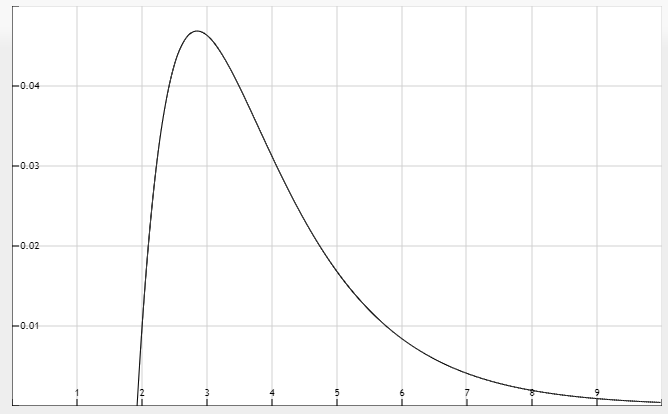
\includegraphics[width=0.9\linewidth]{images/degree_distribution.png}
		\caption{Degree distribution for the given fitness distribution}
		\label{distribution}
	\end{figure}
	
\end{enumerate}